% Options for packages loaded elsewhere
\PassOptionsToPackage{unicode}{hyperref}
\PassOptionsToPackage{hyphens}{url}
\PassOptionsToPackage{dvipsnames,svgnames,x11names}{xcolor}
%
\documentclass[
  letterpaper,
  DIV=11,
  numbers=noendperiod]{scrartcl}

\usepackage{amsmath,amssymb}
\usepackage{iftex}
\ifPDFTeX
  \usepackage[T1]{fontenc}
  \usepackage[utf8]{inputenc}
  \usepackage{textcomp} % provide euro and other symbols
\else % if luatex or xetex
  \usepackage{unicode-math}
  \defaultfontfeatures{Scale=MatchLowercase}
  \defaultfontfeatures[\rmfamily]{Ligatures=TeX,Scale=1}
\fi
\usepackage{lmodern}
\ifPDFTeX\else
    % xetex/luatex font selection
\fi
% Use upquote if available, for straight quotes in verbatim environments
\IfFileExists{upquote.sty}{\usepackage{upquote}}{}
\IfFileExists{microtype.sty}{% use microtype if available
  \usepackage[]{microtype}
  \UseMicrotypeSet[protrusion]{basicmath} % disable protrusion for tt fonts
}{}
\makeatletter
\@ifundefined{KOMAClassName}{% if non-KOMA class
  \IfFileExists{parskip.sty}{%
    \usepackage{parskip}
  }{% else
    \setlength{\parindent}{0pt}
    \setlength{\parskip}{6pt plus 2pt minus 1pt}}
}{% if KOMA class
  \KOMAoptions{parskip=half}}
\makeatother
\usepackage{xcolor}
\setlength{\emergencystretch}{3em} % prevent overfull lines
\setcounter{secnumdepth}{5}
% Make \paragraph and \subparagraph free-standing
\ifx\paragraph\undefined\else
  \let\oldparagraph\paragraph
  \renewcommand{\paragraph}[1]{\oldparagraph{#1}\mbox{}}
\fi
\ifx\subparagraph\undefined\else
  \let\oldsubparagraph\subparagraph
  \renewcommand{\subparagraph}[1]{\oldsubparagraph{#1}\mbox{}}
\fi


\providecommand{\tightlist}{%
  \setlength{\itemsep}{0pt}\setlength{\parskip}{0pt}}\usepackage{longtable,booktabs,array}
\usepackage{calc} % for calculating minipage widths
% Correct order of tables after \paragraph or \subparagraph
\usepackage{etoolbox}
\makeatletter
\patchcmd\longtable{\par}{\if@noskipsec\mbox{}\fi\par}{}{}
\makeatother
% Allow footnotes in longtable head/foot
\IfFileExists{footnotehyper.sty}{\usepackage{footnotehyper}}{\usepackage{footnote}}
\makesavenoteenv{longtable}
\usepackage{graphicx}
\makeatletter
\def\maxwidth{\ifdim\Gin@nat@width>\linewidth\linewidth\else\Gin@nat@width\fi}
\def\maxheight{\ifdim\Gin@nat@height>\textheight\textheight\else\Gin@nat@height\fi}
\makeatother
% Scale images if necessary, so that they will not overflow the page
% margins by default, and it is still possible to overwrite the defaults
% using explicit options in \includegraphics[width, height, ...]{}
\setkeys{Gin}{width=\maxwidth,height=\maxheight,keepaspectratio}
% Set default figure placement to htbp
\makeatletter
\def\fps@figure{htbp}
\makeatother
% definitions for citeproc citations
\NewDocumentCommand\citeproctext{}{}
\NewDocumentCommand\citeproc{mm}{%
  \begingroup\def\citeproctext{#2}\cite{#1}\endgroup}
\makeatletter
 % allow citations to break across lines
 \let\@cite@ofmt\@firstofone
 % avoid brackets around text for \cite:
 \def\@biblabel#1{}
 \def\@cite#1#2{{#1\if@tempswa , #2\fi}}
\makeatother
\newlength{\cslhangindent}
\setlength{\cslhangindent}{1.5em}
\newlength{\csllabelwidth}
\setlength{\csllabelwidth}{3em}
\newenvironment{CSLReferences}[2] % #1 hanging-indent, #2 entry-spacing
 {\begin{list}{}{%
  \setlength{\itemindent}{0pt}
  \setlength{\leftmargin}{0pt}
  \setlength{\parsep}{0pt}
  % turn on hanging indent if param 1 is 1
  \ifodd #1
   \setlength{\leftmargin}{\cslhangindent}
   \setlength{\itemindent}{-1\cslhangindent}
  \fi
  % set entry spacing
  \setlength{\itemsep}{#2\baselineskip}}}
 {\end{list}}
\usepackage{calc}
\newcommand{\CSLBlock}[1]{\hfill\break\parbox[t]{\linewidth}{\strut\ignorespaces#1\strut}}
\newcommand{\CSLLeftMargin}[1]{\parbox[t]{\csllabelwidth}{\strut#1\strut}}
\newcommand{\CSLRightInline}[1]{\parbox[t]{\linewidth - \csllabelwidth}{\strut#1\strut}}
\newcommand{\CSLIndent}[1]{\hspace{\cslhangindent}#1}

\KOMAoption{captions}{tableheading}
\makeatletter
\@ifpackageloaded{caption}{}{\usepackage{caption}}
\AtBeginDocument{%
\ifdefined\contentsname
  \renewcommand*\contentsname{Table of contents}
\else
  \newcommand\contentsname{Table of contents}
\fi
\ifdefined\listfigurename
  \renewcommand*\listfigurename{List of Figures}
\else
  \newcommand\listfigurename{List of Figures}
\fi
\ifdefined\listtablename
  \renewcommand*\listtablename{List of Tables}
\else
  \newcommand\listtablename{List of Tables}
\fi
\ifdefined\figurename
  \renewcommand*\figurename{Figure}
\else
  \newcommand\figurename{Figure}
\fi
\ifdefined\tablename
  \renewcommand*\tablename{Table}
\else
  \newcommand\tablename{Table}
\fi
}
\@ifpackageloaded{float}{}{\usepackage{float}}
\floatstyle{ruled}
\@ifundefined{c@chapter}{\newfloat{codelisting}{h}{lop}}{\newfloat{codelisting}{h}{lop}[chapter]}
\floatname{codelisting}{Listing}
\newcommand*\listoflistings{\listof{codelisting}{List of Listings}}
\makeatother
\makeatletter
\makeatother
\makeatletter
\@ifpackageloaded{caption}{}{\usepackage{caption}}
\@ifpackageloaded{subcaption}{}{\usepackage{subcaption}}
\makeatother
\ifLuaTeX
  \usepackage{selnolig}  % disable illegal ligatures
\fi
\usepackage{bookmark}

\IfFileExists{xurl.sty}{\usepackage{xurl}}{} % add URL line breaks if available
\urlstyle{same} % disable monospaced font for URLs
\hypersetup{
  pdftitle={Bibat: Batteries-include Bayesian Analysis Template},
  pdfauthor={Teddy Groves},
  pdfkeywords={Bayesian workflow, Methodology, Software},
  colorlinks=true,
  linkcolor={blue},
  filecolor={Maroon},
  citecolor={Blue},
  urlcolor={Blue},
  pdfcreator={LaTeX via pandoc}}

\title{Bibat: Batteries-include Bayesian Analysis Template}
\author{Teddy Groves}
\date{}

\begin{document}
\maketitle
\begin{abstract}
Bayesian statistical workflow offers a powerful way to learn from data,
but software software projects that implement complex Bayesian workflows
in practice are unusual, partly due to the difficulty of orchestrating
Bayesian statistical software. Bibat addresses this challenge by
providing a full-featured, scalable Bayesian statistical analysis
project using an interactive template. Bibat is available on the Python
Package index, documented at \url{https://bibat.readthedocs.io/} and
developed at \url{https://github.com/teddygroves/bibat/}. This paper
explains the motivation for bibat, describes intended usage, discusses
bibat's design goals and how key challenges that were overcome in the
course of development, compares bibat with similar software, highlights
several examples of bibat's use in science and provides links to
community resources associated with bibat.
\end{abstract}

\section{Introduction: the problem of orchestrating Bayesian workflow
software}\label{introduction-the-problem-of-orchestrating-bayesian-workflow-software}

The idea that Bayesian statistical analysis comprises not just
inference, but also specific approaches to related activities like data
preparation, model design, diagnosis, debugging and criticism, dates at
least to Box and Tiao (1992). There is increasing scholarly recognition
of the need for a holistic view of ``Bayesian workflow'' (Gelman et al.
2020; Grinsztajn et al. 2021; Gabry et al. 2019). Relatedly, software
tools now exist that address most individual aspects of a Bayesian
workflow: see Štrumbelj et al. (2024) for a review of the state of the
art.

Unfortunately, currently available tools typically address one, or at
most a handful, of Bayesian workflow activities; it is left to the
individual project team to orchestrate the components. Writing software
that performs this orchestration can be time-consuming and tricky,
especially in the common scenario where it is not initially clear how
many, or what kind of, statistical models, datasets, data manipulations
or investigations an analysis will require.

Bibat addresses this difficulty by providing a full-featured,
high-quality Bayesian workflow project that can be extended to implement
a wide range of statistical analyses.

\section{How bibat works}\label{how-bibat-works}

\subsection{Installation and usage}\label{installation-and-usage}

Bibat can be installed on the Windows, Linux or macOS command line on by
running the command \texttt{pip\ install\ bibat} and then used by
running the command \texttt{bibat}. This command triggers an interactive
form which prompts the user to select a range of customisation options.
Bibat then creates a new directory containing code that implements an
example analysis, with customisations reflecting the user's choices.
This analysis works immediately, and can be reproduced with the single
command \texttt{make\ analysis} without the need for any further action
by the user: in this sense bibat comes with batteries included.

Figure~\ref{fig-workflow} illustrates the components of a bibat-based
Bayesian workflow and shows how it proceeds: the project team edits the
code components, then runs \texttt{make\ analysis} triggering creation
of the result components. After inspecting these they repeat the
process, leading to a cycle that ultimately results in a complete,
easily reproducible analysis.

\begin{figure}

\centering{

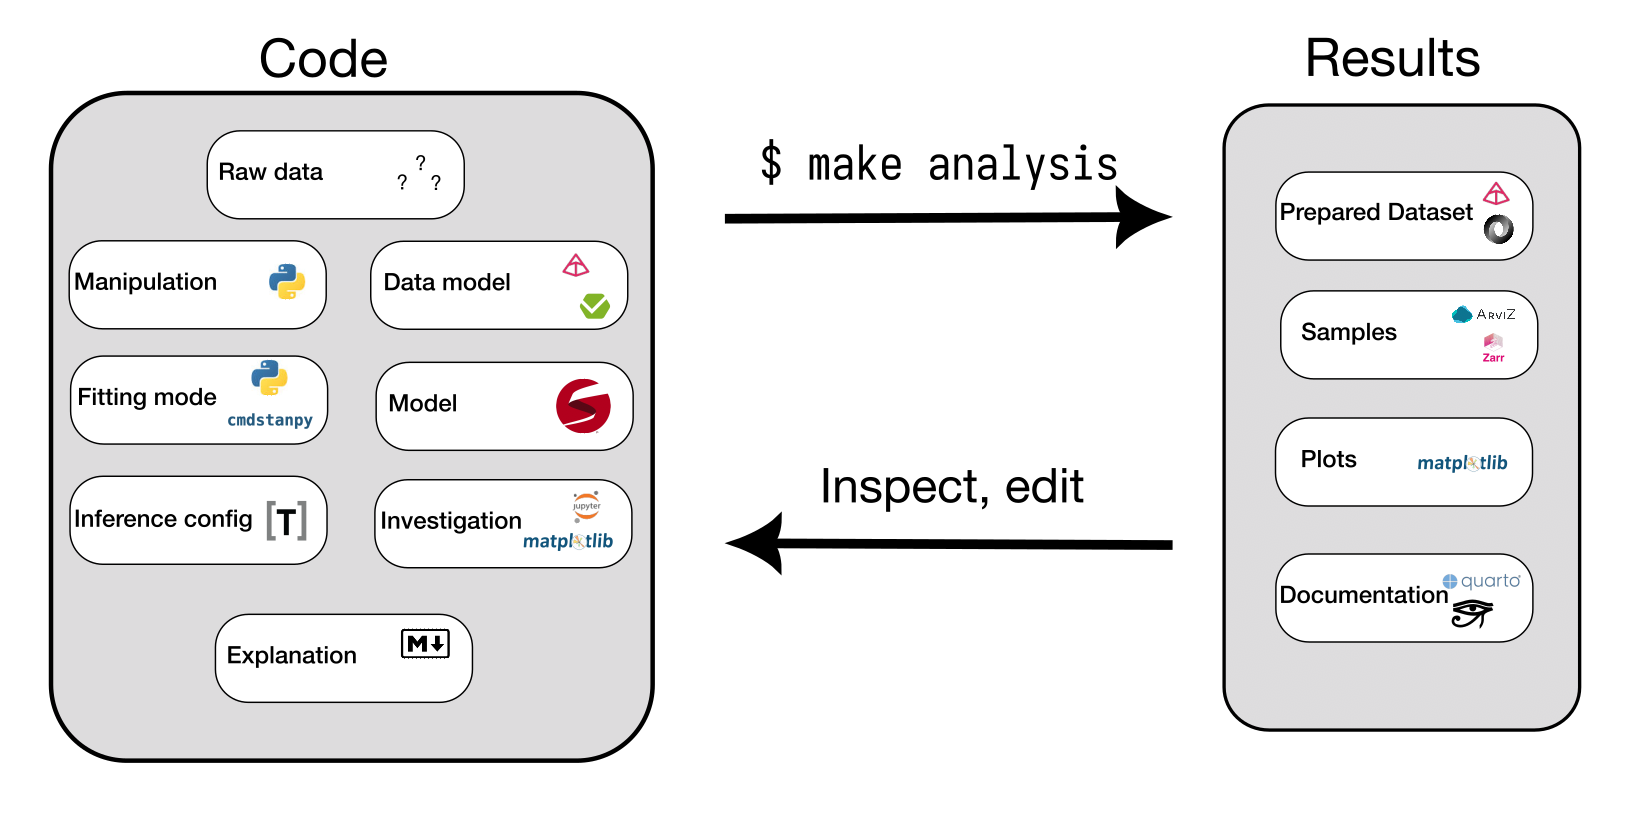
\includegraphics[width=1\textwidth,height=\textheight]{img/workflow.png}

}

\caption{\label{fig-workflow}Schematic representation of a Bayesian
workflow implemented using bibat. The author inspects their analysis's
results, edits code corresponding to the boxes on the left, runs the
command \texttt{make\ analysis}, then repeats. The diagram illustrates
several key features of bibat: inference components are modular and
plural, the overall workflow is iterative and cyclical and the whole
analysis can be executed with a single command.}

\end{figure}%

\subsection{Documentation}\label{documentation}

Bibat is documented at \url{https://github.com/teddygroves/bibat/}. The
documentation website includes instructions for getting started, a
detailed explanation of bibat's concepts and an extended vignette
illustrating how to implement a complex statistical analysis starting
from bibat's example analysis usage. In addition, the documentation site
contains a full description of bibat's python API and command line
interface, instructions for contributing and a section discussing
accessibility considerations.

\section{Design choices}\label{design-choices}

Bibat's design was informed by these considerations.

\subsection{Accommodate a wide range of statistical
analyses}\label{accommodate-a-wide-range-of-statistical-analyses}

Bibat projects explicitly allow for plurality at the level of input
datasets, prepared datasets, statistical models, fitting modes,
computation methods and analyses. In addition, bibat ensures that there
are minimal restrictions on the kind of components: for example,
datasets need not be singular or tabular, and statistical models need
not be representable in formula syntax.

Thanks to these accommodations a project team using bibat should
typically not need to foresee the ultimate requirements of their
analysis before starting the project.

\subsection{Encourage reproducibility}\label{encourage-reproducibility}

Bibat provides a preconfigured makefile with a target \texttt{analysis}
triggering creation of an isolated environment, installation of
dependencies, data preparation, statistical computation and analysis of
results. In this way a bibat analysis can be reproduced on most
platforms using a single command.

In particular, this target attempts to install cmdstan if necessary,
using a recipe tailored to the host operating system. This functionality
addresses a common issue where researchers find it difficult to install
Stan, especially on Windows.

Bibat also provides its Python code in the form of a package configured
using modern conventions for specifying dependencies and configuring
tooling, so that it is easy to maintain reproducibility as the analysis
develops.

\subsection{Use widely-adopted, open source and actively developed
tools}\label{use-widely-adopted-open-source-and-actively-developed-tools}

Bibat projects are is written in modern Python and uses pydantic
Pydantic developers (2022) and pandera (Niels Bantilan 2020) for data
modelling, Stan (Carpenter et al. 2017) for statistical inference,
cmdstanpy (Stan Development Team 2022) for python-Stan interface, arviz
(Kumar et al. 2019) for storing and analyzing inferences and sphinx
(Georg Brandl and the Sphinx team 2022) and quarto (Allaire et al. 2022)
for documentation.

Bibat itself is also written in modern Python and uses the popular tools
cookiecutter (Greenfeld et al. 2021), pydantic and click (Click
Developers 2022).

\subsection{Implement community standards and best practices for
collaborative software
development}\label{implement-community-standards-and-best-practices-for-collaborative-software-development}

Bibat projects include a preconfigured test environment, continuous
integration, linting and pre-commit hooks, making them suitable for
collaborative software development. In addition, including documentation
as a first class component of the analysis addresses a common problem in
academic statistics projects where the paper gets out of sync with the
code.

Bibat itself is continuously tested to ensure that it works on the
operating systems Linux, macOS and Windows. Bibat's continuous
integration runs a test suite as well as an end-to-end functional test
on all supported Python versions.

\section{Challenges}\label{challenges}

This section describes some specific challenges that often affect
Bayesian workflow projects and how bibat addresses them.

\subsection{Address complexity using a modular, file based
approach}\label{address-complexity-using-a-modular-file-based-approach}

As discussed in Gelman et al. (2020), Bayesian workflows are
complicated, featuring plurality, cyclicity and complexity at many
levels. Bibat accommodates this by separating non-interacting analysis
components into modules and by serialising data to files wherever
possible. Prepared datasets, statistical models, inference
configurations, inference results, plots and analyses all have file
representations. Fitting modes, data manipulations and data models are
modularised in code through the use of appropriately structured data
classes and functions.

Thanks to this approach it is possible to perform small sub analyses
individually and to iteratively add components without needing to
consider everything at once.

\subsection{Fitting modes}\label{fitting-modes}

As part of a Bayesian workflow it can be necessary to fit a model and
dataset in different ways. For example, one might perform MCMC sampling
of both the prior and posterior distributions, perform multiple
leave-out-one-fold fits for cross-validation or need to compare MCMC
sampling with an optimisation-based alternative.

Bibat accommodates this need by introducing an abstraction called
``fitting mode''. This abstraction allows bibat projects to handle
fitting a model and dataset in different ways appropriately and
flexibly. For example, the provided prior sampling fitting mode creates
a Stan input dictionary with the \texttt{likelihood} data variable set
to \texttt{0}, performs MCMC sampling and writes data to the
\texttt{InferenceData} group \texttt{prior}. Bibat provides fitting
modes corresponding for prior sampling, posterior sampling and k-fold
posterior sampling. Users can easily add additional fitting modes by
copying these examples.

\section{Comparison with alternative
software}\label{comparison-with-alternative-software}

Other than bibat, there is currently no interactive template that
specifically targets Bayesian workflow projects. There are some
templates that arguably encompass Bayesian workflow as a special case of
data analysis project, such as cookiecutter-data-science (Driven Data
2022), but these are of limited use compared with a specialised template
due to the many specificities of Bayesian workflow.

There is some software that addresses the general task of facilitating
Bayesian workflow, but using a different approach from bibat's. For
example, bambi (Capretto et al. 2020) and brms (Bürkner 2017) aim to
make implementing Bayesian workflows easier by providing ergonomic ways
to specify and fit Bayesian regression models to tabular datasets. Bibat
is complementary with these packages, as it targets use cases that they
do not support, such as analyses where complex datasets or custom models
might be required.

\section{Case studies}\label{case-studies}

The following cases illustrate how bibat has been used in practice to
facilitate Bayesian workflow projects.

Groves and Jooste (2023) used bibat to compare a Bayesian and two
non-Bayesian approaches to modelling a biochemical thermodynamics
dataset. Bibat facilitated this analysis even though it was not very
large---the final analysis contained one dataset, three models and three
inferences---because the fitting mode abstraction allowed for
straightforward comparison of the different methods. Additionally, bibat
made it easier to iteratively investigate and discard models that did
not form part of the final analysis.

In Groves (2022), Bibat was used to implement a sports analysis
involving two datasets, two models and four inferences, demonstrating
that the generalised Pareto distribution can be used to describe hitting
ability in baseball. This analysis is now included in bibat as an
illustration, along with an accompanying tutorial. An illustrative
graphic from this analysis is shown in Figure~\ref{fig-baseball}.

In this case bibat was useful because of its ability to implement
arbitrary statistical models, as latent generalised Pareto distributions
are not supported by generic regression packages like brms and bambi.
Further, bibat's modular design made it easier to implement this
medium-sized analysis with two datasets, two models and six inferences.

\begin{figure}

\centering{

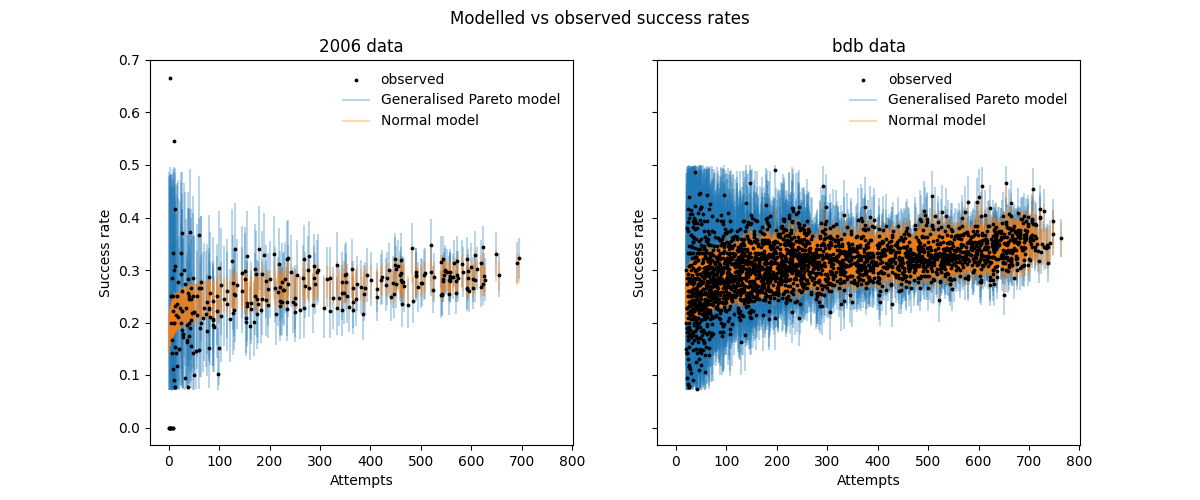
\includegraphics[width=1\textwidth,height=\textheight]{img/baseball.png}

}

\caption{\label{fig-baseball}A graphical posterior predictive check
produced as part of a bibat analysis that fit two statistical models to
two datasets of baseball data. The coloured lines show each model's
posterior predictive distributions and the black dots show the two
observed datasets. See
\url{https://github.com/teddygroves/bibat/tree/main/bibat/examples/baseball}
for the full analysis.}

\end{figure}%

In Groves (2024), bibat was used to implement a large analysis of
cerebrovascular data from mice, involving two raw datasets, 6 prepared
datasets, 15 models and 15 inferences. Again it was not possible to
implement the analysis using formula-based packages due to the need for
custom modelling approaches to take into account expert knowledge about
both the target system and the measurement apparatus. Due to the number
of datasets and models that needed to be considered, implementing this
analysis without using bibat or a similar structured approach would have
required a combination of more time and/ or compromises in software
quality.

These cases illustrate that bibat can be useful in a variety of real
Bayesian workflows, with different sizes, subject matters and emphases.

\section{Community}\label{community}

Bibat is developed in public and encourages community contribution.
Please see the contributing page
\url{https://github.com/teddygroves/bibat/blob/main/CONTRIBUTING.rst}
and code of conduct
\url{https://github.com/teddygroves/bibat/blob/main/CODE_OF_CONDUCT.md}
if you would like to help develop bibat.

Bibat has a growing user community, with 16 GitHub stars at the time of
writing, and is affiliated with cmdstanpy through a link on its
documentation website. Bibat is also affiliated with the Python
scientific software community PyOpenSci, allowing for help with
maintenance as well as peer review for code and documentation quality,
usability and accessibility. The PyOpenSci peer review for bibat can be
found here:
\url{https://github.com/pyOpenSci/software-submission/issues/83}.

\section{Author contributions}\label{author-contributions}

\section*{Acknowledgements}\label{acknowledgements}
\addcontentsline{toc}{section}{Acknowledgements}

\phantomsection\label{refs}
\begin{CSLReferences}{1}{0}
\bibitem[\citeproctext]{ref-Allaire_Quarto_2022}
Allaire, J. J., Charles Teague, Carlos Scheidegger, Yihui Xie, and
Christophe Dervieux. 2022. {``Quarto.''}
\url{https://doi.org/10.5281/zenodo.5960048}.

\bibitem[\citeproctext]{ref-boxBayesianInferenceStatistical1992}
Box, George E. P., and George C. Tiao. 1992. \emph{Bayesian Inference in
Statistical Analysis}. Wiley classics library ed. A {Wiley-Interscience}
Publication. {New York}: {Wiley}.

\bibitem[\citeproctext]{ref-burknerBrmsPackageBayesian2017}
Bürkner, Paul-Christian. 2017. {``Brms: {An R} Package for {Bayesian}
Multilevel Models Using {Stan}.''} \emph{Journal of Statistical
Software} 80 (1): 1--28. \url{https://doi.org/10.18637/jss.v080.i01}.

\bibitem[\citeproctext]{ref-capretto2020}
Capretto, Tomás, Camen Piho, Ravin Kumar, Jacob Westfall, Tal Yarkoni,
and Osvaldo A. Martin. 2020. {``Bambi: {A} Simple Interface for Fitting
{Bayesian} Linear Models in {Python}.''}
\url{https://arxiv.org/abs/2012.10754}.

\bibitem[\citeproctext]{ref-carpenterStanProbabilisticProgramming2017}
Carpenter, Bob, Andrew Gelman, Matthew D. Hoffman, Daniel Lee, Ben
Goodrich, Michael Betancourt, Marcus Brubaker, Jiqiang Guo, Peter Li,
and Allen Riddell. 2017. {``Stan: {A Probabilistic Programming
Language}.''} \emph{Journal of Statistical Software} 76 (1): 1--32.
\url{https://doi.org/10.18637/jss.v076.i01}.

\bibitem[\citeproctext]{ref-clickdevelopersClickPythonComposable2022}
Click Developers. 2022. {``Click: {Python} Composable Command Line
Interface Toolkit.''} Pallets. \url{https://pypi.org/project/click/}.

\bibitem[\citeproctext]{ref-drivendataCookiecutterdatascience2022}
Driven Data. 2022. {``Cookiecutter-Data-Science.''}
\url{https://github.com/drivendata/cookiecutter-data-science/}.

\bibitem[\citeproctext]{ref-gabryVisualizationBayesianWorkflow2019}
Gabry, Jonah, Daniel Simpson, Aki Vehtari, Michael Betancourt, and
Andrew Gelman. 2019. {``Visualization in {Bayesian Workflow}.''}
\emph{Journal of the Royal Statistical Society Series A: Statistics in
Society} 182 (2): 389--402. \url{https://doi.org/10.1111/rssa.12378}.

\bibitem[\citeproctext]{ref-gelmanBayesianWorkflow2020}
Gelman, Andrew, Aki Vehtari, Daniel Simpson, Charles C. Margossian, Bob
Carpenter, Yuling Yao, Lauren Kennedy, Jonah Gabry, Paul-Christian
Bürkner, and Martin Modrák. 2020. {``Bayesian {Workflow}.''}
\emph{arXiv:2011.01808 {[}Stat{]}}, November.
\url{http://arxiv.org/abs/2011.01808}.

\bibitem[\citeproctext]{ref-georgbrandlandthesphinxteamSphinx2022}
Georg Brandl and the Sphinx team. 2022. {``Sphinx.''}
\url{https://www.sphinx-doc.org/}.

\bibitem[\citeproctext]{ref-greenfeldCookiecutter2021}
Greenfeld, Audrey Roy, Dainiel Roy Greenfeld, Raphael Pierzina, et al.
2021. {``Cookiecutter.''} \url{https://pypi.org/project/cookiecutter/}.

\bibitem[\citeproctext]{ref-grinsztajnBayesianWorkflowDisease2021}
Grinsztajn, Léo, Elizaveta Semenova, Charles C. Margossian, and Julien
Riou. 2021. {``Bayesian Workflow for Disease Transmission Modeling in
{Stan}.''} \emph{Statistics in Medicine} 40 (27): 6209--34.
\url{https://doi.org/10.1002/sim.9164}.

\bibitem[\citeproctext]{ref-grovesBaseball2022}
Groves, Teddy. 2022. {``Baseball.''}
\url{https://github.com/teddygroves/baseball}.

\bibitem[\citeproctext]{ref-grovesteddySphincter2024}
---------. 2024. {``Sphincter.''}
\url{https://github.com/teddygroves/sphincter}.

\bibitem[\citeproctext]{ref-grovesteddyDgfreg2023}
Groves, Teddy, and Jason Jooste. 2023. {``Dgfreg.''} DTU Biosustain.
\url{https://github.com/biosustain/dgfreg}.

\bibitem[\citeproctext]{ref-kumarArviZUnifiedLibrary2019}
Kumar, Ravin, Colin Carroll, Ari Hartikainen, and Osvaldo Martin. 2019.
{``{ArviZ} a Unified Library for Exploratory Analysis of {Bayesian}
Models in {Python}.''} \emph{Journal of Open Source Software} 4 (33):
1143. \url{https://doi.org/10.21105/joss.01143}.

\bibitem[\citeproctext]{ref-niels_bantilan-proc-scipy-2020}
Niels Bantilan. 2020. {``Pandera: {Statistical Data Validation} of
{Pandas Dataframes}.''} In \emph{Proceedings of the 19th {Python} in
{Science Conference}}, edited by Meghann Agarwal, Chris Calloway, Dillon
Niederhut, and David Shupe, 116--24.
\url{https://doi.org/10.25080/Majora-342d178e-010}.

\bibitem[\citeproctext]{ref-pydanticdevelopersPydantic2022}
Pydantic developers. 2022. {``Pydantic.''}
\url{https://pypi.org/project/pydantic/}.

\bibitem[\citeproctext]{ref-standevelopmentteamCmdStanPy2022}
Stan Development Team. 2022. {``{CmdStanPy}.''}
\url{https://github.com/stan-dev/cmdstanpy}.

\bibitem[\citeproctext]{ref-strumbeljPresentFutureSoftware}
Štrumbelj, Erik, Alexandre Bouchard-Côté, Jukka Corander, Andrew Gelman,
Håvard Rue, Lawrence Murray, Henri Pesonen, Martyn Plummer, and Aki
Vehtari. 2024. {``Past, {Present}, and {Future} of {Software} for
{Bayesian Inference}.''}

\end{CSLReferences}



\end{document}
